\documentclass[11pt,a4paper]{article}
\usepackage[T1]{fontenc}
\usepackage[utf8]{inputenc}
\usepackage{lmodern}
\usepackage[margin=2.5cm]{geometry}
\usepackage{amsmath,amssymb}
\usepackage{graphicx}
\usepackage{booktabs}
\usepackage{siunitx}
\usepackage[authoryear,round]{natbib}
\usepackage[hidelinks]{hyperref}
\usepackage{xcolor}
\usepackage{caption}
\usepackage{lineno}
\usepackage{setspace}
\sisetup{group-separator={\,}, group-minimum-digits=4}
\captionsetup{font=small,labelfont=bf}
\graphicspath{{figures/}}
\setlength{\emergencystretch}{3em}
\newcommand{\mgal}{\ensuremath{\,\mathrm{mGal}}}
\newcommand{\kgm}{\ensuremath{\,\mathrm{kg\,m^{-3}}}}

\title{A reproducible, test-driven workflow for reducing and gridding legacy gravity compilations with calibrated uncertainty, verified on a synthetic benchmark}
\author{Albert Johan Herrera\\[2pt]
\small Programa de Ingenier\'ia Topogr\'afica y Geom\'atica, Universidad del Quind\'io, Armenia, Colombia\\
\small \texttt{alberthj.herreras@uqvirtual.edu.co} \quad ORCID: 0009-0009-1490-9075}
\date{}

\begin{document}
\maketitle
\linenumbers
\onehalfspacing

\begin{abstract}
Bouguer anomaly maps are routinely built from legacy gravity compilations whose reduction choices, reduction density, curvature term and gridding method are undocumented, inconsistent between subsets and rarely accompanied by uncertainty. We present an open, test-driven workflow that turns such compilations into free-air, simple Bouguer and complete Bouguer anomalies (CBA) of known quality, and verify every step on a deterministic synthetic benchmark with known truth. The reduction follows the North American standard of \citet{Hinze2005}; a legacy mode reproduces spreadsheet formulas exactly, and a term-by-term reconciliation recovers the defects injected into two simulated legacy subsets: a reduction density of $2300\kgm$ (effect up to $-4.2\mgal$) and a supplied curvature term with inverted sign that biases one subset by up to $0.75\mgal$. Nettleton and Parasnis estimators recover a known density within $40\kgm$ on a high-relief survey but fail, and are flagged as unreliable, when the anomaly follows a low-relief topography. Under nested spatial block cross-validation, regression kriging with a Mat\'ern covariance, equivalent sources and a spline reduce the error of inverse-distance weighting by 62--72\,\%; random cross-validation understates these errors by factors of 1.7--5.1. Only kriging provides uncertainty, and once calibrated on inner folds it reaches nominal coverage on held-out blocks (0.956) and against the true field (0.953). Software, benchmark and validation protocol are openly available.
\end{abstract}

\paragraph{Keywords:} Bouguer anomaly; gravity reduction; spherical cap correction; spatial cross-validation; kriging uncertainty; equivalent sources; synthetic benchmark; reproducibility.

\paragraph{Resumen.} Los mapas de anomal\'ia de Bouguer suelen construirse a partir de compilaciones gravim\'etricas heredadas cuyas decisiones de reducci\'on y de interpolaci\'on no est\'an documentadas, difieren entre subconjuntos y carecen de incertidumbre. Se presenta un flujo abierto y verificado por pruebas que transforma tales compilaciones en anomal\'ias de aire libre, de Bouguer simple y de Bouguer completa de calidad conocida, y se verifica cada paso sobre una campa\~na sint\'etica determinista con verdad conocida. La conciliaci\'on t\'ermino a t\'ermino recupera los defectos introducidos en dos hojas de c\'alculo heredadas simuladas: una densidad de reducci\'on de $2300\kgm$ (efecto de hasta $-4{,}2\mgal$) y un t\'ermino de curvatura con signo invertido (sesgo de hasta $0{,}75\mgal$). Los estimadores de Nettleton y Parasnis recuperan una densidad conocida con alto relieve, pero fallan, y se marcan como no fiables, cuando la anomal\'ia sigue una topograf\'ia de bajo relieve. Con validaci\'on cruzada espacial anidada, el kriging de regresi\'on, las fuentes equivalentes y un spline reducen el error de la interpolaci\'on IDW entre 62 y 72\,\%; la validaci\'on cruzada aleatoria subestima esos errores entre 1,7 y 5,1 veces. Solo el kriging entrega incertidumbre, y una vez calibrada alcanza la cobertura nominal en bloques retenidos (0,956) y frente a la verdad (0,953).

\section{Introduction}

Complete Bouguer anomalies (CBA) are the standard input to regional studies of crustal structure and sedimentary basins. Turning observed gravity into a CBA map nevertheless involves a chain of choices: the reference ellipsoid and normal-gravity formula, the treatment of the atmosphere and of the permanent tide, the height correction, the reduction density, the curvature (Bullard B) term, the terrain correction and, finally, the method used to interpolate scattered stations onto a grid. Each choice is well studied individually \citep{LaFehr1991b,Hinze2003,Nowell1999,HackneyFeatherstone2003}, and \citet{Hinze2005} consolidated them into a reduction standard. In practice, however, regional compilations are often assembled from heterogeneous legacy subsets whose reductions differ, whose intermediate quantities are supplied without documentation and whose maps are interpolated over areas with no data.

Interpolation adds its own, frequently ignored, uncertainty. Gravity stations in poorly accessible regions are usually acquired along roads and rivers, producing strongly clustered, line-based sampling. Geostatistical prediction then depends on an admissible covariance model fitted in metric coordinates \citep{Cressie1985,ChilesDelfiner2012}; the Gaussian model, still common in desktop GIS, leads to ill-conditioned systems \citep{Stein1999}. Alternatives such as minimum-curvature splines \citep{Briggs1974,SmithWessel1990,Uieda2018} and equivalent sources \citep{Dampney1969,Cordell1992,SolerUieda2021} are physically or numerically attractive but lack a native error model. Moreover, the usual leave-one-out or random cross-validation is optimistic for autocorrelated, clustered data, and spatially blocked designs are recommended \citep{Roberts2017}. Few gravity studies report calibrated prediction uncertainty or the share of a map that is actually supported by data.

This paper presents a reproducible workflow that addresses these issues and verifies it where the answer is known: on a deterministic synthetic survey with line-based sampling, a known true anomaly, injected data defects and two simulated legacy subsets with undocumented reduction errors. We ask four methodological questions. (Q1) Can a term-by-term reconciliation between legacy and standard reductions detect and attribute undocumented reduction defects? (Q2) When can the reduction density be estimated from the data themselves? (Q3) Which gridding method minimizes the predictive error for line-sampled stations, and can its uncertainty be calibrated on held-out data and against the truth? (Q4) How optimistic is random cross-validation compared with a spatial block design?

Our contributions are: (i) a legacy mode that reproduces spreadsheet formulas exactly and a term-by-term reconciliation that attributes every difference to an individual reduction term; (ii) a nested spatial block cross-validation protocol that selects hyper-parameters and calibrates uncertainty on inner folds and evaluates both on outer folds; (iii) a deterministic synthetic benchmark with known truth, injected defects, simulated legacy subsets and two density scenarios; and (iv) open software with a web interface in which every product carries its provenance.

\section{Methods}

\subsection{Harmonization and quality control}

Records from several subsets are merged by identifier when all principal facts agree within tolerances ($10^{-6}$\,deg, \SI{0.01}{m}, \SI{0.01}{mGal}, $10^{-4}\mgal$ for TC) and flagged otherwise. Stations closer than \SI{1}{m} are merged into one position (mean $g$, $H$ and TC), and the spread of $g$ within merged groups is kept as evidence of repeatability. Quality control never deletes a record; it assigns flags from a controlled vocabulary: schema and range errors, shared-identifier conflicts, duplicate positions, suspect TC (zero at $H>\SI{20}{m}$, or a robust outlier relative to the 10 nearest neighbours, $|z_\mathrm{MAD}|>3.5$; \citealp{RousseeuwHubert2011}), non-positive heights, offshore coordinates, outliers of the free-air--height relation and spatial outliers of the cross-validation residuals. Only error flags remove a station from the grids; suspect TC values are treated as missing, so the affected stations contribute to free-air and simple Bouguer products but not to the CBA grid. The other flags are advisory.

\subsection{Reduction chain}

All corrections are written as values added to the observed gravity, so that every anomaly is $g+\sum\delta g-\gamma_0$. Normal gravity on the GRS80 ellipsoid \citep{Moritz2000} uses Somigliana's closed form,
\begin{equation}
\gamma_0(\varphi)=\gamma_e\,\frac{1+k\sin^2\varphi}{\sqrt{1-e^2\sin^2\varphi}},
\end{equation}
with $\gamma_e=978\,032.67715\mgal$, $k=0.001\,931\,851\,353$ and $e^2=0.006\,694\,380\,022\,90$. Following \citet{Hinze2005}, the free-air, simple Bouguer and complete Bouguer anomalies are
\begin{align}
\mathrm{FAA}&=g+g_H-\gamma_0+\delta g_h+\delta g_\mathrm{atm},\\
\mathrm{SBA}&=\mathrm{FAA}-2\pi G\rho H,\\
\mathrm{CBA}&=\mathrm{FAA}-BC_\mathrm{cap}(H,\rho)+\mathrm{TC}\,\rho/\rho_\mathrm{TC},
\end{align}
where $g_H=0.0371(1-3\sin^2\varphi)$ is the Honkasalo term that removes the permanent-tide correction of IGSN71 data, $\delta g_\mathrm{atm}=0.874-9.9\times10^{-5}H+3.56\times10^{-9}H^2$, $\delta g_h=(0.3087691-0.0004398\sin^2\varphi)H-7.2125\times10^{-8}H^2$ (all in mGal with $H$ in metres), $G=6.67430\times10^{-11}\,\mathrm{m^3\,kg^{-1}\,s^{-2}}$ \citep{Tiesinga2021}, and $BC_\mathrm{cap}$ is the attraction of a spherical cap of radius \SI{166.735}{km} in the closed form of \citet{LaFehr1991a}. The curvature term is $BB=BC_\mathrm{cap}-2\pi G\rho H$; it is positive below about \SI{4.15}{km}, so it reduces the anomaly. The reference density is $2670\kgm$ \citep{Hinze2003}.

The implementation was verified against analytical golden values (normal gravity to $10^{-4}\mgal$; other terms to $10^{-5}\mgal$), against the GRS80 implementation of the Boule library \citep{Boule} to better than $10^{-3}\mgal$ from pole to pole, and against the cubic approximation of the curvature term \citep{Whitman1991}, which it matches to $5\times10^{-4}\mgal$ below \SI{300}{m}. Property-based tests check the identity $\mathrm{CBA}=\mathrm{SBA}-BB+\mathrm{TC}_\rho$ to $10^{-9}\mgal$.

\subsection{Legacy mode and term-by-term reconciliation}

Legacy spreadsheets typically combine a hard-coded slab density, a first-order height correction ($0.3086H$), their own normal-gravity coefficients and a curvature value supplied per station without documentation of its sign convention. The legacy mode reproduces such formulas exactly, so that the cached legacy anomalies can be verified before they are compared with the standard ones. The reconciliation then computes both reductions with all intermediate terms and decomposes the difference into normal gravity, Honkasalo, atmospheric, height, slab-density, curvature and terrain-scaling contributions; the sum of the contributions must close the total difference to numerical precision. The supplied curvature values are also compared with the recomputed $BB$: a correct ``value to add'' has a ratio close to $-1$, whereas a ratio close to $+1$ reveals an inverted sign.

\subsection{Station uncertainty}

Station uncertainty is propagated to first order from independent errors in $g$ ($\sigma_g=\SI{0.1}{mGal}$ by default), $H$ (\SI{1}{m}), TC (10\,\%) and horizontal position (\SI{50}{m}), using central-difference derivatives of the full reduction (e.g.\ $\partial\mathrm{CBA}/\partial H=0.195\mgal\,\mathrm{m^{-1}}$ for $2670\kgm$). A Monte Carlo propagation (2\,000 draws) with common random numbers and moment matching verifies the linear values. The density is treated as a scenario, not as a random error.

\subsection{Density diagnostics}

The Nettleton estimate minimizes $|\mathrm{corr}(\mathrm{CBA}(\rho),H)|$ over $1800$--$3000\kgm$, and the Parasnis estimate is the least-squares slope of FAA on the unit-density Bouguer-plus-terrain term $X=BC_\mathrm{cap}(H;1\kgm)-\mathrm{TC}/\rho_\mathrm{TC}$ \citep{Nettleton1939,Parasnis1952}. Both are computed on residuals of a degree-2 polynomial trend to suppress regional correlation, with 95\,\% intervals from a spatial block bootstrap (\SI{15}{km} blocks, 1\,000 replicates). An estimate is considered reliable only if both interval half-widths are below $300\kgm$, the estimate is physically plausible and the two intervals overlap.

\subsection{Spatial model and gridding}

All spatial computations use projected metric coordinates (EPSG:9377; \citealp{IGAC2020}). The gridded anomaly is modelled as
\begin{equation}
Z(\mathbf{s})=m(\mathbf{s})+Y(\mathbf{s})+\varepsilon(\mathbf{s}),
\end{equation}
where $m$ is a polynomial drift of degree $p\in\{0,1,2\}$, $Y$ a zero-mean Gaussian process with Mat\'ern covariance
\begin{equation}
C(r)=\sigma^2\frac{2^{1-\nu}}{\Gamma(\nu)}\left(\frac{\sqrt{2\nu}\,r}{\ell}\right)^{\nu}K_\nu\!\left(\frac{\sqrt{2\nu}\,r}{\ell}\right),\qquad \nu\in\{0.5,1.5,2.5\},
\end{equation}
and $\varepsilon$ a nugget of variance $\tau^2$. The Gaussian covariance is excluded \citep{Stein1999}. Covariance parameters are fitted by weighted least squares to the experimental semivariogram of the drift residuals \citep{Cressie1985} (bins of \SI{1.5}{km}, lags up to \SI{30}{km}), with a fixed fallback sequence. Prediction is by regression kriging (OLS drift and simple kriging of the residuals); its variance is reported raw and multiplied by a calibration factor $c=\mathrm{sd}(z)$ obtained from block cross-validation, where $z=(Z_\mathrm{obs}-\hat Z)/\hat\sigma$. Geometric anisotropy is modelled only if the minor/major ratio of directional length scales is below 0.7 in at least four of five folds. The gridding methods compared are inverse-distance weighting (IDW, power 2, 12 neighbours, a common legacy choice), a linear trend plus a biharmonic spline \citep{Uieda2018}, equivalent sources at relative depths of 7--\SI{20}{km} with damping 0.01--1 \citep{SolerUieda2021,Harmonica}, and regression kriging. Grids have \SI{500}{m} cells \citep{Hengl2006}; cells farther than \SI{5}{km} from a station or outside the convex hull are masked as unsupported.

\subsection{Validation design}

Hyper-parameters (drift degree and $\nu$ for kriging; depth and damping for equivalent sources) and the calibration factor are selected on inner five-fold spatial block cross-validation within each training set of an outer five-fold block cross-validation (\SI{15}{km} blocks). The outer folds therefore provide honest estimates of predictive error (RMSE) and of calibration (sd$(z)$ and the share of $|z|<1.96$). The sensitivity of the conclusions to the fold layout and block size is assessed with two further random seeds and with 10- and 25-km blocks. For comparison, the same nested protocol is repeated with \SI{250}{m} blocks, which contain at most one station each and are therefore equivalent to random five-fold cross-validation.

\subsection{Software and reproducibility}

The workflow is implemented as a typed Python package (\texttt{gravanom}) built on NumPy, xarray, pyproj, Verde \citep{Uieda2018}, Harmonica \citep{Harmonica}, Boule \citep{Boule} and GSTools \citep{Muller2022}, with a FastAPI service and a MapLibre web interface. About 170 automated tests cover formulas, quality-control rules, the pipeline, the API and eight end-to-end acceptance scenarios. Every run writes a manifest with input and output hashes, the resolved configuration, package versions and seeds; repeated runs produce byte-identical tables and grids.

\section{Synthetic benchmark}

The benchmark is generated deterministically from a fixed seed (Fig.~\ref{fig:survey}). A topography with heights of 5--\SI{269}{m} (mean \SI{142}{m}) and a terrain-correction field of 0.1--\SI{1.0}{mGal} are drawn as Mat\'ern random fields over a $160\times\SI{160}{km}$ square. The true CBA, from $-68$ to $-10\mgal$, is the sum of a quadratic regional field and the attraction of four buried prisms with density contrasts of $-300$, $-200$, $+150$ and $+250\kgm$, tops at 5.5--\SI{7.9}{km} depth and widths of 10--\SI{25}{km}, computed with Harmonica at the topographic surface. Two thousand stations are placed on 20 meandering traverses with a spacing of 1.0--\SI{1.6}{km}, leaving gaps of tens of kilometres between lines. Observed gravity is obtained by inverting the standard reduction exactly with $\rho_\mathrm{true}=2670\kgm$, so that the noise-free observations reduce to the true CBA; Gaussian noise of \SI{0.3}{mGal} is added to gravity and of \SI{1}{m} to the reported heights. Five duplicate positions (two with a \SI{0.5}{mGal} offset), three terrain corrections set to zero above \SI{50}{m} and one gross gravity error are injected, giving 2\,005 records.

Two legacy subsets, A and B, are simulated from the 1\,996 clean stations by splitting them into even and odd traverses (997 and 999 stations). Both are reduced with typical legacy spreadsheet formulas: slab density $2300\kgm$, first-order height correction and legacy normal-gravity coefficients. Subset A supplies the cubic approximation of the curvature term with the correct ``value to add'' sign; subset B supplies it with the opposite sign and 8\,\% too large. Two further variants test the density estimators: a high-relief survey (0--\SI{1500}{m}, $\rho_\mathrm{true}=2400\kgm$) and a low-relief survey in which the true anomaly contains a term of $0.08\mgal\,\mathrm{m^{-1}}$ proportional to the topography, mimicking lowlands that coincide with thick, light sedimentary fill.

\begin{figure}[t]
\centering
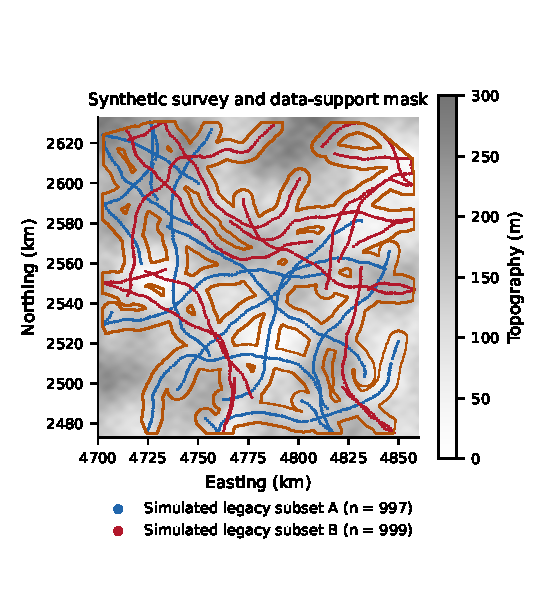
\includegraphics[width=0.55\textwidth]{fig01_survey.pdf}
\caption{Synthetic survey: topography, stations of the two simulated legacy subsets (even and odd traverses) and the data-support mask (orange: cells within \SI{5}{km} of a station and inside the convex hull). All values are fictitious.}
\label{fig:survey}
\end{figure}

\section{Results}

\subsection{Quality control and station uncertainty}

Quality control flags all nine injected defects: the five duplicate positions are merged (the two offset pairs imply a repeatability of $\sigma_g\approx\SI{0.22}{mGal}$), the three zero terrain corrections are flagged as suspect and the gross error is flagged as out of range. The remaining 1\,996 stations enter the CBA grid. Advisory flags mark 38 stations whose fictitious coordinates fall offshore, 31 spatial outliers of the cross-validation residuals and seven outliers of the free-air--height relation; none of them is removed. With the default error budget, the median station uncertainty is \SI{0.32}{mGal} for the FAA and \SI{0.23}{mGal} for the CBA, dominated by the height error, and the Monte Carlo and linear values agree to better than $10^{-6}$ (relative).

\subsection{Reconciling legacy and standard reductions (Q1)}

The legacy mode reproduces the simulated spreadsheets exactly, and the term-by-term decomposition closes the difference between the standard CBA ($\rho=2670\kgm$) and the legacy CBA to $2.3\times10^{-10}\mgal$ (Table~\ref{tab:terms}). The reduction density dominates: replacing $2300$ by $2670\kgm$ changes the CBA by $-2.15\mgal$ on average and by up to $-4.08\mgal$ at the highest stations (Fig.~\ref{fig:legacy}a). The curvature contribution separates the two subsets. For subset A it is zero within $3	imes10^{-4}\mgal$, and the ratio of supplied to recomputed curvature is $-0.999$, the correct convention. For subset B the ratio is $+1.079$, which reveals both the inverted sign and the 8\,\% excess (Fig.~\ref{fig:legacy}b), and the curvature term contributes $-0.40\mgal$ on average and up to $-0.71\mgal$. Consequently, even with the density fixed at the legacy $2300\kgm$, the standard CBA differs from legacy A by only $-0.04\mgal$ on average (range $-0.10$ to $+0.03$), whereas it differs from legacy B by $-0.42\mgal$ on average and by up to $-0.75\mgal$. The height correction contributes about $+0.02\mgal$, and the legacy normal-gravity coefficients reproduce GRS80 to $10^{-5}\mgal$.

\begin{table}[t]
\centering\small
\caption{Term-by-term decomposition of the difference between the standard CBA ($\rho=2670\kgm$) and the CBA of the two simulated legacy subsets (mGal). Injected defects: density $2300\kgm$ in both subsets; curvature with inverted sign and 8\,\% excess in subset B.}
\label{tab:terms}
\begin{tabular}{lrrrr}
\toprule
 & \multicolumn{2}{c}{Subset A} & \multicolumn{2}{c}{Subset B} \\
Term & Mean & Min & Mean & Min \\
\midrule
Slab density (2670 vs 2300) & $-2.31$ & $-4.16$ & $-2.10$ & $-3.87$ \\
Curvature (supplied vs recomputed) & $0.00$ & $0.00$ & $-0.40$ & $-0.71$ \\
Height correction & $+0.02$ & $0.00$ & $+0.02$ & $0.00$ \\
Total difference & $-2.29$ & $-4.12$ & $-2.47$ & $-4.54$ \\
\midrule
Standard ($\rho=2300$) minus legacy & $-0.04$ & $-0.10$ & $-0.42$ & $-0.75$ \\
Ratio supplied/recomputed BB & \multicolumn{2}{c}{$-0.999$} & \multicolumn{2}{c}{$+1.079$} \\
\bottomrule
\end{tabular}
\end{table}

\begin{figure}[t]
\centering
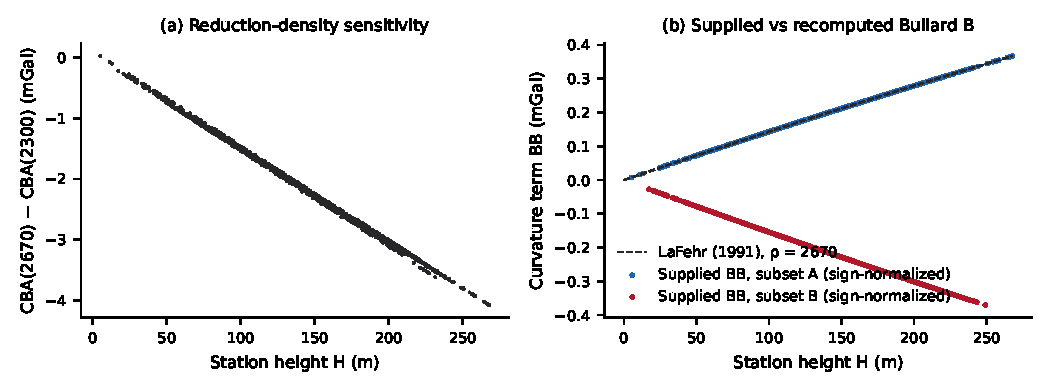
\includegraphics[width=\textwidth]{fig02_legacy.pdf}
\caption{(a) Change of the CBA when the reduction density is raised from 2300 to $2670\kgm$, as a function of station height. (b) Curvature term recomputed with the LaFehr closed form compared with the values supplied with the two simulated legacy subsets (sign-normalized to the ``value subtracted'' convention): subset A coincides with the recomputed term, subset B has the opposite sign and is 8\,\% too large.}
\label{fig:legacy}
\end{figure}

\subsection{Density diagnostics (Q2)}

On the high-relief survey (height sd \SI{285}{m}), Nettleton gives $2440\kgm$ (95\,\% interval 2340--2570) and Parasnis $2437\kgm$ (2342--2570), both containing the true $2400\kgm$, and the reliability criterion is met (Fig.~\ref{fig:density}). On the low-relief survey whose anomaly follows the topography (height sd \SI{46}{m}), the Nettleton criterion reaches the upper bound of the search range and Parasnis gives a physically implausible $4\,110\kgm$ (3\,394--4\,839), although the true density is $2670\kgm$. Removing a quadratic trend does not help, because the correlation between anomaly and topography is local. The reliability criterion correctly rejects both estimates, so the workflow falls back to the conventional density and reports the alternative as a scenario.

\begin{figure}[t]
\centering
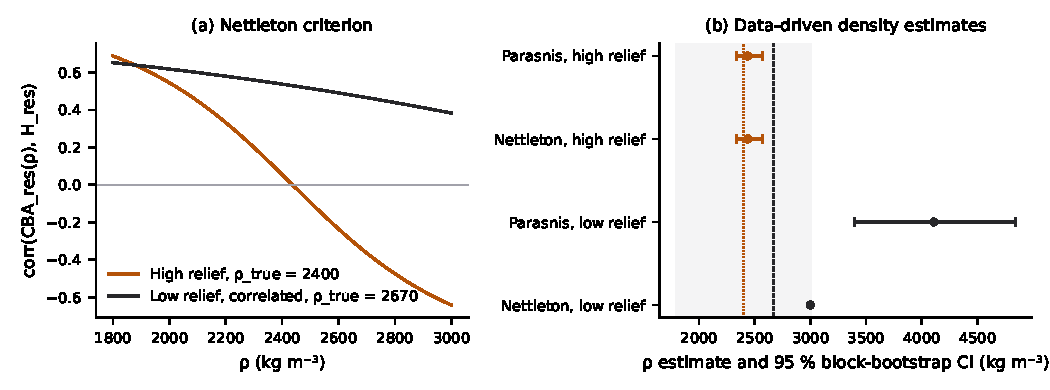
\includegraphics[width=\textwidth]{fig03_density.pdf}
\caption{(a) Nettleton criterion for the high-relief survey ($\rho_\mathrm{true}=2400\kgm$) and for the low-relief survey whose anomaly follows the topography ($\rho_\mathrm{true}=2670\kgm$). (b) Nettleton and Parasnis estimates with 95\,\% block-bootstrap intervals; the shaded band marks physically plausible densities.}
\label{fig:density}
\end{figure}

\subsection{Variography and gridding performance (Q3, Q4)}

The experimental semivariogram of the drift residuals is well described by a Mat\'ern model with $\nu=1.5$, a length scale of \SI{46}{km}, a partial sill of \SI{137}{mGal^2} and a nugget of \SI{0.10}{mGal^2} on a degree-2 drift (Fig.~\ref{fig:variogram}). Directional length scales differ: the minor/major ratio is below 0.7 in four of the five outer folds (0.55--0.77), so the anisotropy test is positive (major axis N45$^\circ$E, ratio 0.64) and the anisotropic model competes with isotropic ones in the inner selection; it was chosen in one fold.

\begin{figure}[t]
\centering
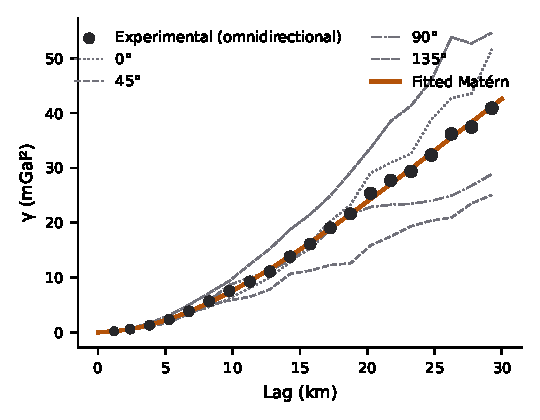
\includegraphics[width=0.55\textwidth]{fig04_variogram.pdf}
\caption{Experimental semivariogram of the CBA drift residuals (marker size proportional to the number of pairs), directional semivariograms and the fitted Mat\'ern model ($\nu=1.5$).}
\label{fig:variogram}
\end{figure}

Under outer spatial block cross-validation (Table~\ref{tab:cv}, Fig.~\ref{fig:validation}), the trend-plus-spline has the lowest error (\SI{0.69}{mGal}), followed by regression kriging (\SI{0.74}{mGal}) and equivalent sources (\SI{0.94}{mGal}); IDW is clearly worst (\SI{2.49}{mGal}). The three model-based methods therefore reduce the IDW error by 62--72\,\%, and their differences are comparable to the spread between folds. The ratio of kriging to IDW error is stable across fold layouts (0.27--0.36 for three seeds) and block sizes (0.31 and 0.34 for 10- and 25-km blocks). Only kriging delivers an uncertainty estimate. Its raw variance is conservative (sd$(z)=0.84$), and after scaling with the inner-fold factor ($c=0.73$) the outer-fold calibration is close to nominal (sd$(z)=0.90$, 95\,\% coverage 0.956); it remains so for all seeds and block sizes (coverage 0.956--0.972). Random cross-validation is markedly optimistic: it understates the error of IDW by a factor of 5.1, of equivalent sources by 2.5, of kriging by 2.0 and of the spline by 1.7, and it would rank the methods differently.

\begin{table}[t]
\centering\small
\caption{Outer five-fold cross-validation of the CBA on the synthetic survey (1\,996 stations): spatial blocks of \SI{15}{km} and the random-equivalent design. Hyper-parameters and calibration were selected on inner folds.}
\label{tab:cv}
\begin{tabular}{lrrrrr}
\toprule
Method & Block RMSE & Fold RMSE & Random RMSE & sd$(z)$ & 95\,\% cov. \\
\midrule
IDW ($p=2$, $k=12$) & 2.49 & $2.42\pm0.63$ & 0.49 & -- & -- \\
Linear trend + biharmonic spline & 0.69 & $0.69\pm0.11$ & 0.40 & -- & -- \\
Equivalent sources & 0.94 & $0.89\pm0.32$ & 0.38 & -- & -- \\
Regression kriging (Mat\'ern) & 0.74 & $0.72\pm0.15$ & 0.38 & 0.90 & 0.956 \\
\bottomrule
\end{tabular}
\end{table}

\begin{figure}[t]
\centering
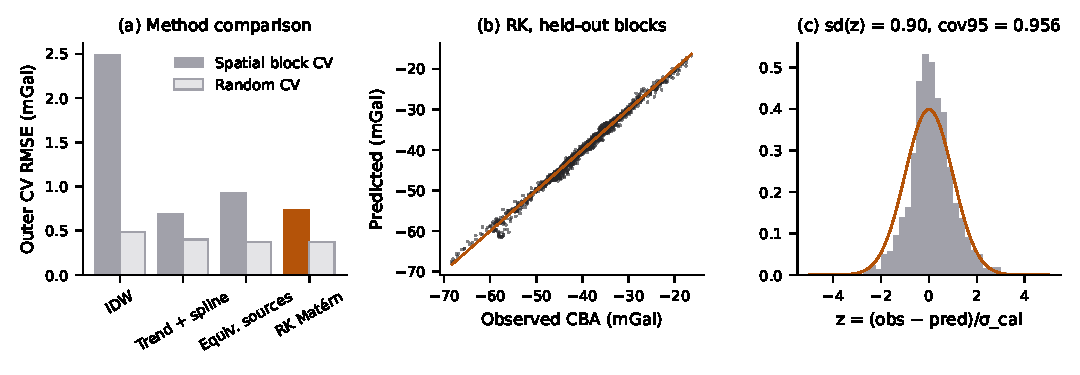
\includegraphics[width=\textwidth]{fig05_validation.pdf}
\caption{(a) Outer cross-validation RMSE of the four methods with spatial blocks and with the random-equivalent design. (b) Predicted versus observed CBA at held-out stations for regression kriging. (c) Standardized errors with calibrated uncertainty and the standard normal density.}
\label{fig:validation}
\end{figure}

\subsection{Truth recovery and data support}

Inside the support mask, the kriging grid differs from the true field by \SI{0.27}{mGal} RMS, well below the cross-validation estimate, because most supported cells lie close to a traverse, whereas the outer folds predict whole blocks (Fig.~\ref{fig:truth}). The calibrated uncertainty covers the true field at the nominal rate (95\,\% coverage 0.953); it has a median of \SI{0.24}{mGal} and grows to \SI{1.0}{mGal} towards the gaps between traverses and the edges of the mask. The support mask retains 65\,\% of the square; the remaining area is extrapolation and is not published. The cell size has a negligible effect: the RMS difference between a \SI{250}{m} grid and the bilinearly resampled \SI{500}{m} grid is \SI{0.002}{mGal}.

\begin{figure}[t]
\centering
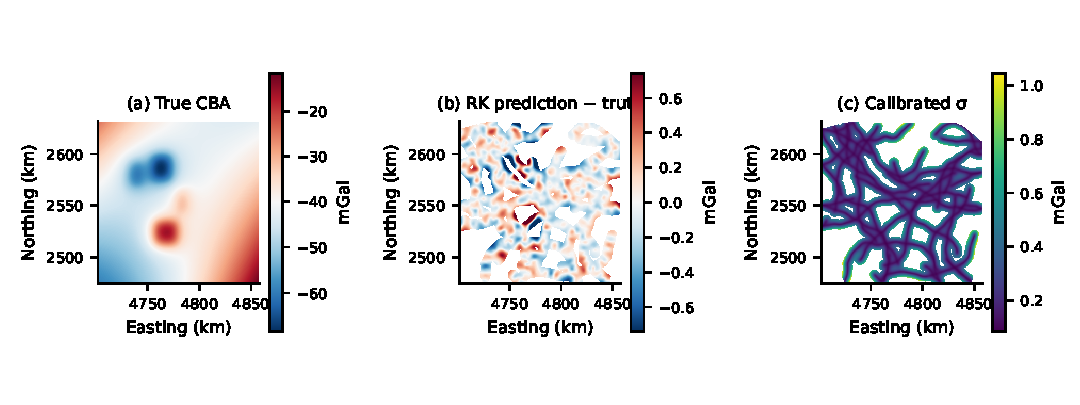
\includegraphics[width=\textwidth]{fig06_truth.pdf}
\caption{Synthetic benchmark: (a) true CBA at the topographic surface; (b) kriging prediction minus truth inside the support mask (RMSE \SI{0.27}{mGal}); (c) calibrated prediction uncertainty.}
\label{fig:truth}
\end{figure}

\section{Discussion}

\paragraph{What legacy reductions hide.} The reconciliation shows that two maps computed from the same observations can differ by several mGal for reasons unrelated to geology: the reduction density and a curvature term whose sign and magnitude depend on how it was supplied. Each of these choices is small compared with the amplitude of regional anomalies, but together they exceed the station uncertainty by an order of magnitude and are spatially structured, since they scale with height. A single comparison of the final anomalies would mix both effects; the term-by-term decomposition, which closes to numerical precision, separates them and identifies the defective subset, and the ratio of supplied to recomputed curvature exposes a sign convention that is otherwise invisible. Reproducing the legacy numbers exactly, rather than only recomputing ``correct'' anomalies, is therefore a prerequisite for merging compilations.

\paragraph{When the density cannot be estimated.} Data-driven density estimates assume that the anomaly is uncorrelated with the topography after the regional trend is removed. The low-relief variant shows that this assumption fails precisely in sedimentary basins, where lowlands coincide with thick, light fill: both estimators then return biased values with narrow or implausible intervals. A reliability rule that combines interval width, physical plausibility and agreement between methods prevents such estimates from being used silently.

\paragraph{Validation of gridded products.} The comparison of gridding methods depends strongly on the validation design. Random cross-validation of line-sampled data mostly tests interpolation between neighbouring stations of the same traverse and understates the error of predicting across the gaps, most severely for IDW. With a spatial block design, the three model-based methods perform similarly and their ranking should not be over-interpreted. The decisive difference is uncertainty: equivalent sources and splines provide no error model, whereas kriging, once its variance is calibrated by an inner-fold factor, produces prediction intervals with nominal coverage both on unseen blocks and against the true field. Following \citet{Stein1999}, the Gaussian covariance was excluded; together with weighted least-squares fitting in metric coordinates, this prevents the ill-conditioning and the non-admissible variogram curves that occur when variograms are fitted by polynomials in geographic degrees.

\paragraph{Limitations.} The benchmark tests the workflow where the truth is known, but it cannot reproduce every difficulty of real compilations: undocumented gravity datums and height systems, terrain corrections computed with unknown methods, drift and tares of individual surveys, and correlated errors between stations of the same campaign. The simulated legacy defects are representative but not exhaustive. Ellipsoidal heights would allow gravity disturbances \citep{LiGotze2001,HackneyFeatherstone2003}; terrain corrections could be verified with a digital elevation model and prism modelling \citep{Nagy2000}; and global models such as EGM2008 \citep{Pavlis2012} or XGM2019e \citep{Zingerle2020}, distributed by ICGEM \citep{Ince2019}, would allow a consistency check of long wavelengths when the workflow is applied to real data. Regional--residual separation by upward continuation \citep{Jacobsen1987}, edge detection \citep{BlakelySimpson1986} and spectral depth estimates \citep{SpectorGrant1970} are natural extensions.

\section{Conclusions}

A reproducible, test-driven workflow turns heterogeneous legacy gravity subsets into anomalies and grids of known quality, and a synthetic benchmark with known truth verifies each step. (1) A legacy mode and a term-by-term reconciliation recover undocumented reduction defects exactly: the effect of a $2300\kgm$ slab density (up to \SI{4.1}{mGal}) and a supplied curvature term with inverted sign (bias up to \SI{0.75}{mGal}) are attributed to the correct term and subset. (2) Nettleton and Parasnis estimators recover a known density on a high-relief survey but fail when the anomaly follows a low-relief topography; a reliability rule flags these cases. (3) Under spatial block cross-validation, kriging, equivalent sources and splines reduce the IDW error by 62--72\,\%, and only kriging provides uncertainty that is calibrated both on held-out blocks and against the truth. (4) Random cross-validation understates gridding errors by factors of 1.7--5.1 for line-sampled stations. Spatially blocked validation, calibrated uncertainty and data-support masks should therefore accompany every published Bouguer anomaly grid.

\section*{Data and code availability}
The software (\texttt{gravanom}, API and web interface), the synthetic benchmark, the validation protocol and the scripts that generate every figure and number of this article are available at \url{https://github.com/alberttkd/static-gravity-anomalies-colombia} under the BSD-3-Clause licence (documentation and synthetic data: CC BY 4.0). All data used in this article are synthetic and can be regenerated from the published seeds.

\section*{CRediT authorship contribution statement}
\textbf{Albert Johan Herrera:} Conceptualization, Methodology, Software, Validation, Formal analysis, Investigation, Data curation, Writing -- original draft, Writing -- review \& editing, Visualization.

\section*{Declaration of competing interest}
The author declares no competing financial interests or personal relationships that could have influenced the work reported in this paper.

\section*{Declaration of generative AI and AI-assisted technologies}
During the preparation of this work the author used Claude (Anthropic), an AI assistant, to support software development and testing and the drafting and editing of the text. The author reviewed and edited all content and takes full responsibility for the publication.

\section*{Funding}
This research did not receive any specific grant from funding agencies in the public, commercial or not-for-profit sectors.

\bibliographystyle{abbrvnat}
\bibliography{references}

\end{document}
